\chapter{Learning Rappresentation}
Uno degli obiettivi del Deep Learning è imparare rappresentazioni significative a partire da dei dati grezzi. Un buon modello di Deep Learning, non si limita a classificare gli input, ma è in grado di estrarre delle caratteristiche gerarchiche le quali semplificano notevolmente i compiti di analisi e previsione.

\section{Classificatori Lineari e i loro Limiti}
I classificatori lineari, visti durante il corso di Machine Learning, suddividono lo spazio degli input in due regioni separate tramite un iperpiano. Questa soluzione però risulta essere molto limitata per due motivi:
\begin{itemize}
    \item Non è in grado di gestire problemi con dati non linearmente separabili;
    \item La probabilità che una distribuzione casuale di punti $P$ sia separabile linearmente diminuisce all'aumentare della dimensionalità $N$ nel momento in cui $P \ge N$ (Teorema di Cover, 1966).
\end{itemize}

Se provassimo ad aumentare la dimensione di $N$ per cercare di arginare il problema, a causa del teorema di Cover dobbiamo non ignorare la problematica della \textit{Curse of Dimensionality}, la quale è anch'essa campo di studio.

\begin{figure}[!ht]
    \centering
    \begin{subfigure}[b]{0.45\textwidth}
        \centering
        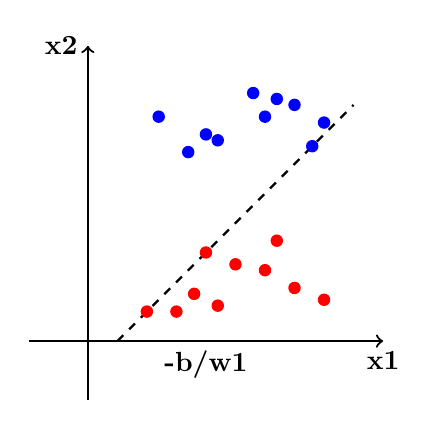
\begin{tikzpicture}[scale=0.75]
            \draw[->, thick] (-1,0) -- (5,0) node[anchor=north] {\textbf{x1}};
            \draw[->, thick] (0,-1) -- (0,5) node[anchor=east] {\textbf{x2}};
            \node[below] at (2,0) {\textbf{-b/w1}};
            \draw[thick, dashed] (0.5,0) -- (4.5,4);
            \foreach \x/\y in {
                2/3.5, 1.2/3.8, 3.5/4, 2.8/4.2, 4/3.7,
                3.8/3.3, 3.2/4.1, 2.2/3.4, 3/3.8, 1.7/3.2
            } {
                \fill[blue] (\x,\y) circle (3pt);
            }
            \foreach \x/\y in {
                1/0.5, 2/1.5, 1.8/0.8, 3/1.2, 4/0.7,
                2.5/1.3, 3.5/0.9, 1.5/0.5, 3.2/1.7, 2.2/0.6
            } {
                \fill[red] (\x,\y) circle (3pt);
            }
        \end{tikzpicture}
        \caption{Dati linearmente separabili}
    \end{subfigure}
    \hfill
    \begin{subfigure}[b]{0.45\textwidth}
        \centering
        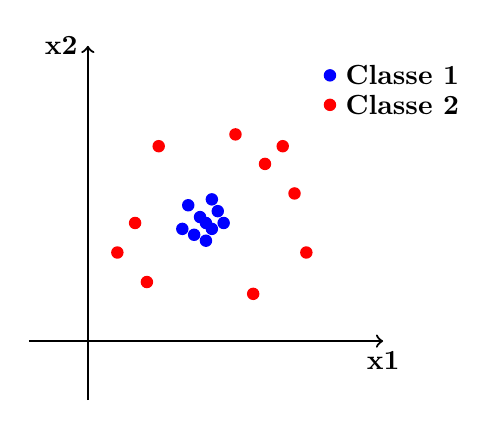
\begin{tikzpicture}[scale=0.75]
            \draw[->, thick] (-1,0) -- (5,0) node[anchor=north] {\textbf{x1}};
            \draw[->, thick] (0,-1) -- (0,5) node[anchor=east] {\textbf{x2}};
            \foreach \x/\y in {
                2/2, 2.2/2.2, 1.8/1.8, 2.1/1.9, 1.9/2.1,
                2/1.7, 2.3/2, 1.7/2.3, 2.1/2.4, 1.6/1.9
            } {
                \fill[blue] (\x,\y) circle (3pt);
            }
            \foreach \x/\y in {
                1/1, 3/3, 3.5/2.5, 2.5/3.5, 1.2/3.3,
                3.7/1.5, 0.8/2, 3.3/3.3, 2.8/0.8, 0.5/1.5
            } {
                \fill[red] (\x,\y) circle (3pt);
            }
            \fill[blue] (4.1,4.5) circle (3pt);
            \node[right] at (4.2,4.5) {\textbf{Classe 1}};
            \fill[red] (4.1,4) circle (3pt);
            \node[right] at (4.2,4) {\textbf{Classe 2}};
        \end{tikzpicture}
        \caption{Dati non linearmente separabili}
    \end{subfigure}

    \caption{Confronto tra un dataset linearmente separabile (a sinistra) e uno non linearmente separabile (a destra).}
    \label{fig:linear-vs-non-linear}
\end{figure}

\subsection{La funzione XOR}
Per superare i limiti dei classificatori lineari, si adottano diverse metodologie, una di queste è approfondita attraverso la funzione \textbf{XOR}, vista nel corso di Machine Learning, dove per definizione la funzione XOR genera dei dati che non sono linearmente separabili, ma attraverso la combinazione di modelli più semplici, riusciamo a ottenere la funzione complessiva attraverso una rete neurale con esiti linearmente separabili. Di seguito alcune metodologie per far fronte ai limiti dei classificatori lineari:
\begin{itemize}
    \item Estrarre caratteristiche rilevanti dall'input grezzo;
    \item Trasformare i dati in una rappresentazione in cui la separabilità lineare sia più semplice;
    \item Usare estrattori di caratteristiche non lineari, come reti neurali profonde.
\end{itemize}

\section{Metodi di Estrazione}
Alcuni metodi per estrarre caratteristiche utili includono:
\begin{itemize}
    \item \textbf{Tiling dello spazio:} suddivisione dello spazio in regioni più piccole;
    \item \textbf{Proiezioni casuali:} trasformazioni casuali per aumentare la dimensione dello spazio;
    \item \textbf{Classificatori polinomiali:} utilizzo di combinazioni di variabili di input per migliorare la separabilità;
    \item \textbf{Macchine a kernel}: mappatura non lineare dei dati in uno spazio a più alta dimensionalità.
\end{itemize}

L'idea alla base di tutte queste possibilità è quella di poter espandere le dimensioni della nostra rappresentazione, portando i nostri dati ad essere lineramente separabili con facilità.

\begin{Osservazione}
    Utilizzare le features in maniera lineare, risulta essere più semplice a livello di costo computazionale.
\end{Osservazione}

\section{Reti Neurali Poco Profonde}
Per poter far fronte a questa problematica, si possono utilizzare le strategie quì di seguito elencate:

\begin{itemize}
    \item Le macchine a vettori di supporto (SVM) e i metodi a kernel utilizzano uno strato con funzioni di base non lineari, seguito da uno strato lineare;
    \item Utilizzare delle reti neurali con due strati diventando degli approssimatori universali~\ref{th:Cybenko_1989}, tuttavia richiedono un numero elevato di neuroni per rappresentare funzioni complesse.
\end{itemize}

\begin{Teorema}
    Una rete con 2 strati (con 1 strato nascosto), è un approssimatore universale, può approssimare in modo arbitrariamente preciso ogni funzione continua $g(u_1,u_2,\dots,u_d)$.
    \label{th:Cybenko_1989}
\end{Teorema}

A fronte di questo teorema potremmo chiederci del perché con il Deep Learning, utilizziamo delle reti neurali più profonde, visto che ogni funzione continua è rappresentabile con un singolo layer nascosto.

\subsubsection{Perché le Architetture Profonde?}
Una rete neurale profonda è in grado di rappresentare funzioni complesse in modo più efficiente rispetto a una rete non profonda. Nel momento in cui passiamo a una rete neurale profonda otterremo un risultato in meno tempo, dunque si rinuncia a dello spazio per risparmiare del tempo. Inoltre esse hanno:
\begin{itemize}
    \item Maggiore capacità di modellare strutture gerarchiche nei dati  (es. riconoscimento visivo, riconosco una figura a seconda di sue diverse caratteristiche, ognuna analizzata in un layer);
    \item Possibilità di apprendere trasformazioni sempre più astratte dei nostri dati.
\end{itemize}

\section{Ipotesi del Manifold}
Un concetto molto importante del Deep Learning è l'ipotesi del \textbf{Manifold}. Il nostro obbiettivo vuole essere quello di riconoscere la faccia della persona presente nella Figura~\ref{fig:manifold}, notiamo come in ognuna delle sottofigure vi è la stessa persona, noi riusciamo a caprilo facilmente, ma come questo accade ci permette di comprendere come potrebbero farlo le macchine. Ci sono delle caratteristiche che siamo in grado di riconoscere le quali appartengono alla stessa persona. Il nostro cervello, e più in generale, la nostra realtà si trova in uno spazio dimensionale che non è della stessa grandezza di una figura che possiamo creare.

\begin{figure}[h]
    \centering
    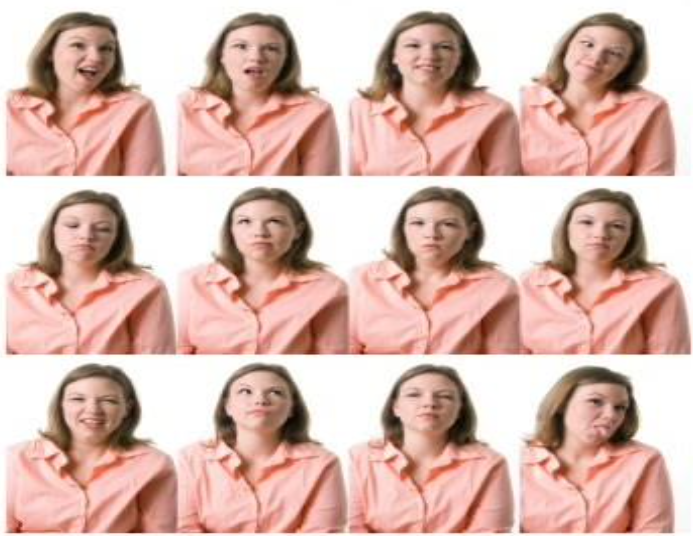
\includegraphics[width=0.45\textwidth]{figure/Manifold.png}
    \caption{Esempio dell'ipotesi del manifold.}
    \label{fig:manifold}
\end{figure}

\marginpar{L'argomento della Data Manifold, viene trattato meglio in: \href{https://ieeexplore.ieee.org/stamp/stamp.jsp?tp=&arnumber=1640964}{Hadsell et al. CVPR 2006~\cite{hadsell2006dimensionality}}}

È stato dimostrato come noi umani, siamo in grado di riconoscere una faccia di una persona rappresentando meno di 56 variabili, mentre un calcolatore usando un'immagine $1000$x$1000$ pixel avrò bisogno di $1\,000\,000$ di variabili. Questa è la così detta ipotesi del Manifold: la realtà vive in una dimensione notevolmente minore rispetto alla dimensione che utiliziamo per rappresentarla, differentemente da ciò che avviene per le macchine. 

\subsubsection{Correlazione con cio che stiamo facendo}
Se avessimo un estrattore ideale, potremmo essere in grado di prendere questa immagine da un milione di dimensioni, ed estrarre le 56 features, in modo tale da essere in grado di riconoscere l'immagine. Rappresentando i cambiamenti su un piano cartesiano, spostandoci lungo una singola dimensione cambieremo solo ed esclusivamente una singola features (Figura~\ref{fig:cartesianFig}).

\begin{figure}
    \centering
    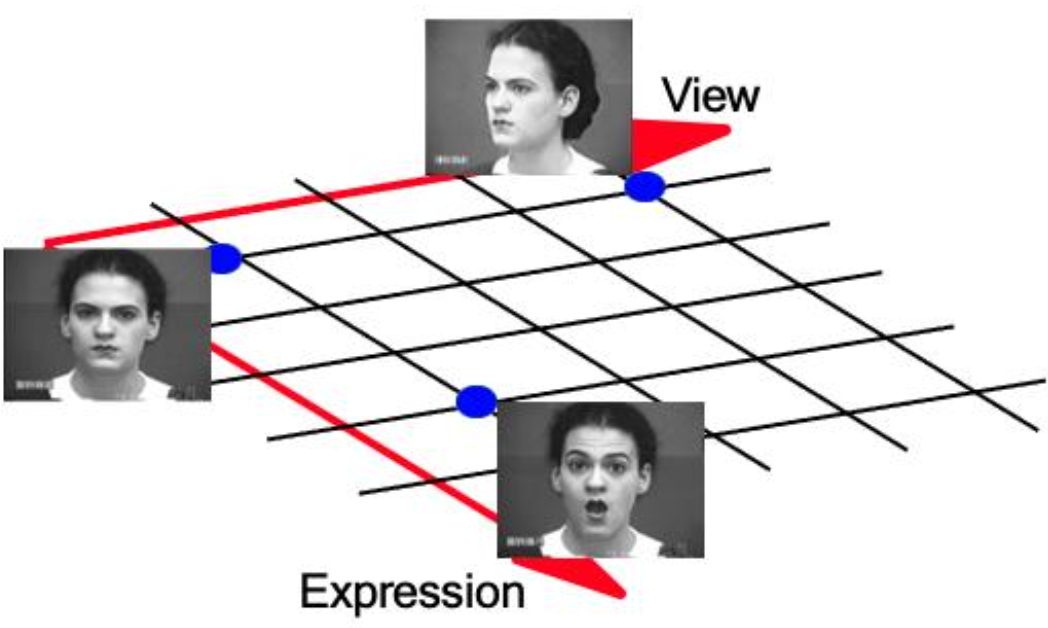
\includegraphics[width=0.45\linewidth]{figure/cartesianFig.png}
    \caption{Rappresentazione di un estrattore ideale di features su un piano cartesiano.}
    \label{fig:cartesianFig}
\end{figure}
\section{Struttura Gerarchica dei Dati}
Le architetture multilivello riflettono la natura composizionale dei dati, analizzando parti dei dati ogni volte, queste possono diventare delle ottime possibilità per spostarci verso un estrattore ideale, permettendo un'efficiente rappresentazione delle informazioni:

\begin{itemize}
    \item \textbf{Visione:} pixel $\Rightarrow$ bordi $\Rightarrow$ texture $\Rightarrow$ oggetti;
    \item \textbf{Testo:} caratteri $\Rightarrow$ parole $\Rightarrow$ frasi $\Rightarrow$ discorso;
    \item \textbf{Audio:} campioni $\Rightarrow$ bande spettrali $\Rightarrow$ fonemi $\Rightarrow$ parole.
\end{itemize}

\section{Conclusione}
Le reti neurali profonde permettono di bilanciare tempo e spazio, garantendo che i più livelli implichino più operazioni sequenziali, riducono la necessità di risorse computazionali parallele e consentono una rappresentazione più compatta delle funzioni complesse.